\section{Illustration}
%\section{Experimentations}

To illustrate our theoretical results, we evaluate the predictive performance and the ability of the models to capture homophily and preferential attachment on artificial and real networks. In the sequel, we first describe the measures used to evaluate the properties of interest and the predictive performance, then the datasets used in our experiments. Afterwards, we detail the evaluation protocol and we present the experimental results.


\subsection{Preferential attachment Measures}
\label{sec:experiments-burst}

The measures considered to evaluate the preferential attachment rely on a goodness of fit. Indeed, it has been reported that preferential attachment leads to networks characterized by a degree distribution with heavy tail drawn from a power law \textbf{ref?}. A graphical method, most often used to verify that the observations are consistent with this law  consists in constructing the histogram representing the degree distribution and if the plot on doubly logarithmic axes approximately falls on a straight line, then one can assume that the distribution follows a power law. Thus, the comparison of the degree distribution in the log-log scale with a linear function gives us a qualitative measure for the preferential attachment. To obtain a second evaluation of the power law hypothesis for the degree distribution, we follow the statistical framework, introduced by \cite{clauset2009power}, for discerning and quantifying power-law behavior in empirical data. This framework combines maximum-likelihood fitting methods with goodness-of-fit tests based on the Kolmogorov-Smirnov statistic. It includes the following steps:


\begin{itemize}
	\item Estimate the parameters $\alpha$ and $x_\text{min}$ of the power law model. $\alpha$ is the scaling parameter of the law and $x_\text{min}$, the lower bound for the tail. It has been fixed to the smallest value observed in the distributions evaluated, in our experiments to allow their comparisons.
	\item  Using the Kolmogorov-Smirnov (KS) statistic, compute the distance $KS_{obs}$  between the degree distribution obtained on the network with the theoretical distribution corresponding to the power law with the estimated parameters.
	\item Sample $S$ synthetic datasets from the power law with the estimated parameters. For each sample s, using the Kolmogorov-Smirnov statistic, compute the distance $KS_{s}$ between the distribution obtained on this synthetic dataset drawn from the power law with the corresponding theoretical distribution. According to  \cite{clauset2009power}, the number of samples $S$ is chosen such that $S = \frac{1}{4}\epsilon^{-2}$, with a precision  $\epsilon = 3^{-2}$ \textbf{a revoir}. 
    \item  The p-value is defined as the fraction of  the resulting statistics $KS_s, s \in \{1,...,S\}$ obtained on the samples larger than the value $KS_{obs}$ computed on the network distribution.  
\end{itemize}

 If  p-value is large (close to 1), then the difference between the data and the model can be attributed to statistical fluctuations alone; if it is small, the model is not a plausible fit for the data and we can not conclude that there is an evidence for the preferential attachment in the network. 
\textbf{arevoir}However, as mentioned in \cite{clauset2009power} high value of the $p$-value should be considered with caution for at least two reasons. First, there may be other distribution that match the data equally or better. Second, a small number of samples of the data may lead to high p-value and reflect the fact that is hard to rule out a hypothesis in such a case.


\paragraph{Local burstiness : }
%In the context of latent models, while there is no ambiguity in computing the overall degree distribution, it is less obvious for the local case. We explain here the computation of the local degree distribution for each models according to section \ref{sec:burstiness} :
The computation of the local degree distribution for each model defined according to section \ref{sec:burstiness} is detailed below: 
\begin{itemize}
        \item For each network learned with IMMSB, the tensor $Z$ indicates the membership of the nodes for each  interaction. In order to draw the local degree distribution for a factor $k$, we reduce the adjacency matrix in order to retain only the links that occur for the factor $k$. The local degree distribution is thus computed on the reduced adjacency matrix  $Y^k =\{ y_{ij}^k=1 \ \textrm{if}\ y_{ij}=1 , z_{i\rightarrow j}=k, z_{i\leftarrow j}=k\}$. \textbf{termes a 0}
        \item for ILFM, each node $i$ is associated with a fix feature vector $\mat{f}_{i}$ ; the local degree distribution for the factor $k$ is obtained by taking into account only the contribution of this feature $k$ on the adjacency matrix. Thus, the local degree degree distribution is computed on the reduced adjacency matrix defined by $Y^c =\{ y_{ij}^c=1 \ \textrm{if}\ y_{ij}=1 , f_{ic}=1, f_{jc}=1\ }$. \textbf{termes a 0}
\end{itemize}

\subsection{Homophily Measures}

For the homophily property, defined in section \ref{sec:homophily}, we represent using a boxplot, for each model and each data set, the distributions of the similarity natural $s_n(i,j)$ and latent $s_l(i,j)$ computed respectively on linked and non-linked pairs of nodes for 10 networks generated with the model learned on the dataset.
% The links or non-links are obtained by running the models in a generative mode. For each models we aggregated  the similarity of each couple of nodes as well as link prediction (links or non-links). The distributions of similarities are then represented on a boxplot that shows how the they are spread according to links and non-links.

\subsection{Prediction performance evaluation}
The prediction problem is equivalent to a binary prediction problem in two classes since it consists to decide for each pair of nodes if there is an edge or not between them. 
Thus, the performance of the models can be evaluated with usual AUC-ROC measures: Receiver operating characteristic curves allow to graphically compare the predictive performance of the models on each datasets.

\subsection{Training Datasets}

In our experiments, we consider two artificial networks and two real networks.  Main topological characteristics of these networks are summarized in Table \ref{table:networks_measures} and we describe those networks in the sequel.

\begin{table}[h] 
	\centering
	\caption{Characteristics of artificial and real networks.}
	%\resizebox{\textwidth}{!}{  
    \begin{tabular}{lrrr}
        \hline
        \textbf{Networks} &   nodes &   edges &   density \\
        \hline
        Network 1 &    1000 &    3507 &     0.007 \\
        Network 4 &    1000 &   31000 &     0.062 \\
        Blogs         &    1490 &   20512 &     0.009 \\
        Manufacturing &     167 &    5950 &     0.215 \\
    \hline
    \end{tabular}
	\label{table:networks_measures}
\end{table}

The artificial networks have been generated with DANC-Generator \cite{largeron2015}. This generator has been chosen because it allows to build an attributed graph having a community structure  and  the known properties of real-world networks such as preferential attachment and homophily.
Moreover, by modifying the parameters, these properties can be weakened. Finally, DANC-Generator is available under the terms of the GNU Public License and the parameters can be shared for experiments reproducibility. \textcolor{red}{Heeere, words about my platform (pymake) to share and reproduce and create new experiments}.

Two artificial networks (Network1 and Network4) have been generated. Their adjacency matrices and global degree distributions are presented in Figure \ref{fig:corpuses}. Table \ref{table:me_gofit} gives the resulting $p$-value of the KS test as well as the  values estimated for the parameters  $\alpha$ and $x_\text{min}$,  and  the number $n_{tail}$ of observations in the distribution such as $x \geq x_\text{min}$ . For each network, Figure \ref{fig:synt_graph_local} represents the local degree distribution associated to each \emph{ground truth} community and Table \ref{table:me_gofit} reports the KS results in the local case. The inner degree distribution (edges inside a community) and outer degree distribution (edges between community) are plotted separately.

Each network presents a different affinity to preferential attachment and homophily.
Indeed, As shown Figure \ref{fig:corpuses}, Network1 verify the  preferential attachment whereas it is not the case for Network4. The results of the KS test given in Table \ref{table:me_gofit} confirm this analysis since the $p$-value is very high for Network1 and low for Network4, respectively equals to 1 and 0.

Concerning the local preferential attachment, that can be evaluated on these artificial networks where the ground truth communities are provided by the generator, the local degree distributions per class are given in Figure \ref{fig:synt_graph_local} and the average results (and variances) for the p-value computed over the classes are reported in Table \ref{table:me_gofit}. They show that the local preferential attachment is verified the first networks and in a lesser extend for the second. In particularly, the high variance of the $p$-value for Network3 and Network4 indicates that the property varies among the classes. (not reported here).

We evaluated also the models on two real world networks.
The first one, denoted Blogs \footnote{available at: http://moreno.ss.uci.edu/data.html\#blogs}, contains front-page hyperlinks between blogs in the context of the 2004 US election. A node represents a blog and an edge represents a hyperlink between two blogs.
The second one, denoted Manufacturing \footnote{available at: https://www.ii.pwr.edu.pl/~michalski/index.php?content=datasets\#manufacturing}, is an internal email communication network between employees of a mid-sized manufacturing company. Each vertex is associated  to an employee and an oriented link represents like previously a sent email.

The adjacency matrices and global degree distributions are presented in Figure \ref{fig:corpuses}. The goodness of fit based on the KS test, used as a reference for the global preferential attachment effect, is reported in Table \ref{table:me_gofit}. According to Figure \ref{fig:corpuses} as well as Table \ref{table:me_gofit}, it appears that the preferential attachment property is verified in Blogs, with a high p-value, and not in Manufacturing where the p-value is null. As the ground truth is not available for these networks, the local preferential attachment can not be verified.


\begin{figure}[h]
        \begin{minipage}{0.24\textwidth}
            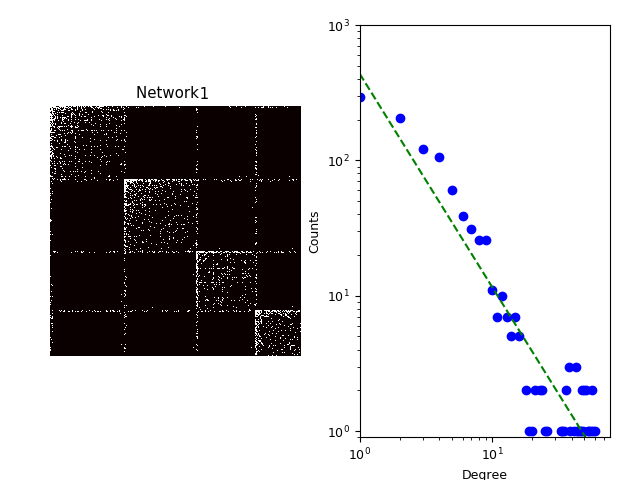
\includegraphics[width=\textwidth]{img/corpus/network1_dd}
        \end{minipage}
        \begin{minipage}{0.24\textwidth}
            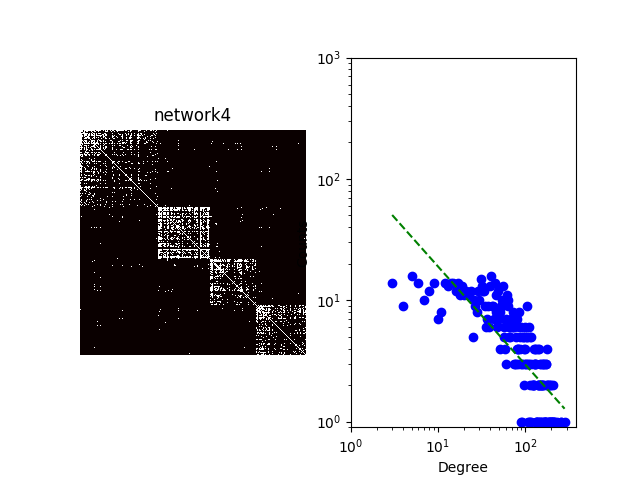
\includegraphics[width=\textwidth]{img/corpus/network4_dd}
        \end{minipage}
        \vskip\baselineskip
        \begin{minipage}{0.24\textwidth}
            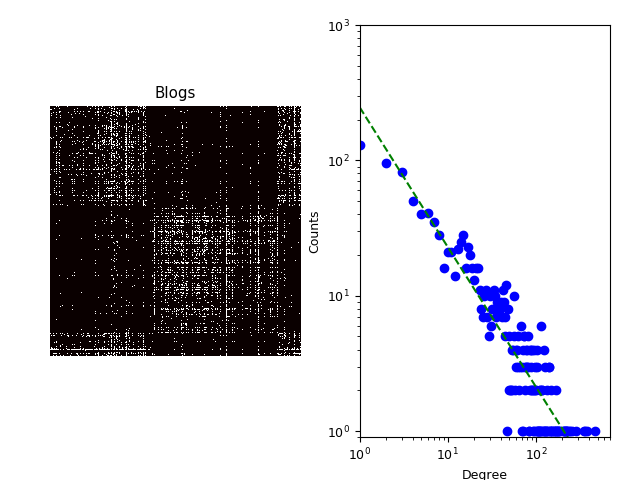
\includegraphics[width=\textwidth]{img/corpus/blogs_dd}
        \end{minipage}
        \begin{minipage}{0.24\textwidth}
            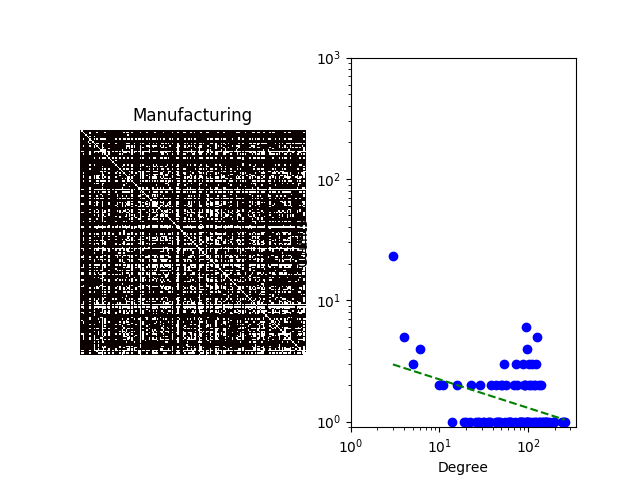
\includegraphics[width=\textwidth]{img/corpus/manufacturing_dd}
        \end{minipage}
	\caption{Adjacency matrices (left) and global degree distributions (right) for the networks datasets.}
	\label{fig:corpuses}
\end{figure}


\begin{figure}[h]
        \begin{minipage}{0.24\textwidth}
            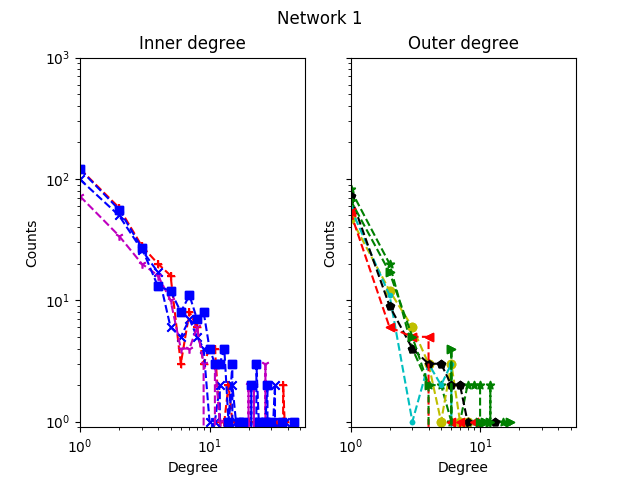
\includegraphics[width=\textwidth]{img/corpus/network1_1}
        \end{minipage}
        \begin{minipage}{0.24\textwidth}
            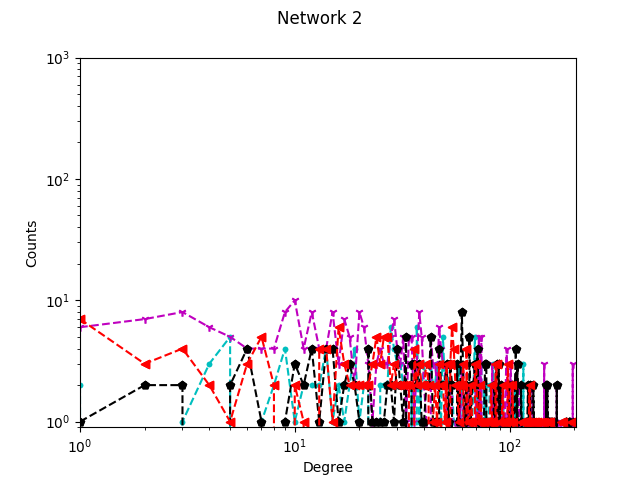
\includegraphics[width=\textwidth]{img/corpus/network2_1}
        \end{minipage}
        \vskip\baselineskip
        \begin{minipage}{0.24\textwidth}
            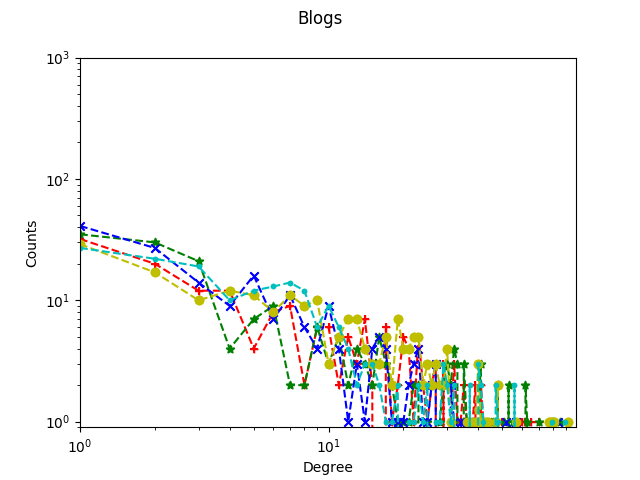
\includegraphics[width=\textwidth]{img/corpus/blogs_1}
        \end{minipage}
        \begin{minipage}{0.24\textwidth}
            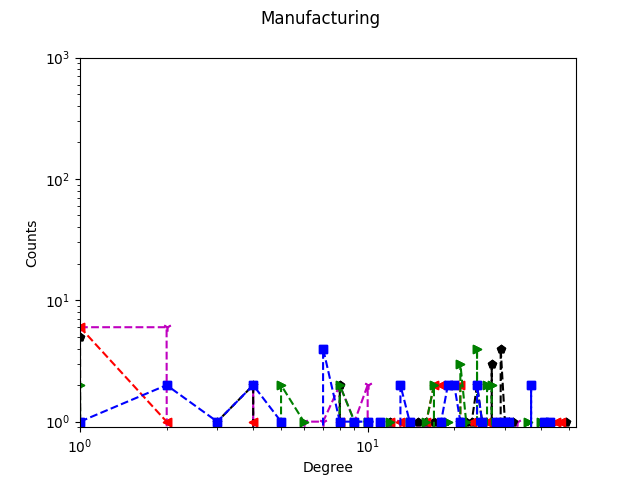
\includegraphics[width=\textwidth]{img/corpus/manufacturing_1}
        \end{minipage}
        \caption {Local degree distributions for the four networks datasets. Inner(left) and outer(right) degree are separated. For Network1 and Network2 the classes come from ground-truth. For Blogs and Manufacturing we use classes find by a Louvain algorithms.} 
	\label{fig:synt_graph_local}
\end{figure}




\subsection{Model Evaluation}
For each dataset described earlier, we run a MCMC inference consisting of 200 iterations to learn the posterior distribution for the IMMSB and ILFM  models described in section \ref{sec:models}. For IMMSB, the concentration parameters of HDP were optimized according to  \cite{HDP} using vague gamma priors $\alpha_0 \sim \text{Gamma}(1,1)$ and $\gamma \sim \text{Gamma}(1,1)$. The parameters for the matrix weights were fixed to $\lambda_0=\lambda_1=0.1$. For ILFM, the IBP hyper-parameter was fixed to $\alpha=0.5$ and the weights hyper-parameter to $\sigma_w = 1$. 

The inference procedure was run with these settings for the four datasets networks previously described.

All our experimental platform is available online \footnote{https://github.com/dtrckd/pymake}. It is an ongoing development in order to provide a flexible way to design and share and make experiments data analysis.

We report in table \ref{table:me_gofit} the value of the power-law goodness of fit as described earlier for a 10 random generated networks with the models fitted on all four dataset. This table shows that the IMMSB comply with the preferential attachment with a maximal pvalue for each datasets while ILFM obtain low pvalue for the networks that were less locally bursty with a value of 0.5 and 0.3 for respectively Network4 and Manufacturing. Also, the mean value of the power-law coefficient $\alpha$ is significantly greater for IMMSB on all dataset with stronger value on the strongest locally bursty networks, Network1 and Blogs.

The figure \ref{fig:me_local} illustrate the local preferential attachments by plotting the averaged local degree distribution of the generated networks. It shows that the shape of local degree distribution appears more bursty for IMMSB and with more fluctuation for ILFM.


\begin{table}[t]
    \caption{Power law goodness of fit results for the preferential attachment for empirical data and fitted models.}
\centering
  \begin{tabular}{lrrrr}
      \multirow{2}{*}{\textbf{Empirical}}  &
      \multicolumn{2}{c}{Global} & \multicolumn{2}{c}{Local}\\
      \cmidrule(r){2-3} \cmidrule(l){4-5}
      &   pvalue &   alpha   & pvalue & alpha   \\
  	\hline
    Network 1     &    1.0 &   2.4 & 1.0 $\pm$ 0.0  &  2.4 $\pm$ 0.5  \\
    Network 4     &    0.0 &   1.3 & 0.6 $\pm$ 0.5  &  1.5 $\pm$ 0.2 \\
    Blogs         &    1.0 &   1.5 & 1.0 $\pm$ 0.   &  1.7 $\pm$ 0.3 \\
    Manufacturing &    0.0 &   1.4 & 0.5 $\pm$ 0.2  &  1.4 $\pm$ 0.1 \\
  	\hline

      \ \textbf{IMMSB} &&&& \\
  	\hline
    Network 1     & 0.9 \(\pm\) 0.1   & 1.4 \(\pm\) 0.0 & 1.0 \(\pm\) 0.0   & 2.9 \(\pm\) 1.4 \\
    Network 4     & 0.0 \(\pm\) 0.0   & 1.3 \(\pm\) 0.1 & 1.0 \(\pm\) 0.0   & 1.8 \(\pm\) 0.2 \\
    Blogs         & 1.0 \(\pm\) 0.0   & 1.3 \(\pm\) 0.0 & 1.0 \(\pm\) 0.0   & 4.5 \(\pm\) 0.9 \\
    Manufacturing & 0.0 \(\pm\) 0.1   & 1.2 \(\pm\) 0.0 & 1.0 \(\pm\) 0.1   & 1.8 \(\pm\) 0.2 \\
  	\hline

      \ \textbf{ILFM} &&&& \\
  	\hline
    Network 1     & 1.0 \(\pm\) 0.0 & 1.4 \(\pm\) 0.0 & 1.0 \(\pm\) 0.0 & 1.8 \(\pm\) 0.3 \\
    Network 4     & 0.0 \(\pm\) 0.0 & 1.2 \(\pm\) 0.0 & 0.5 \(\pm\) 0.5 & 1.3 \(\pm\) 0.1 \\
    Blogs         & 1.0 \(\pm\) 0.0 & 1.3 \(\pm\) 0.0 & 1.0 \(\pm\) 0.0 & 1.5 \(\pm\) 0.1 \\
    Manufacturing & 0.0 \(\pm\) 0.0 & 1.2 \(\pm\) 0.0 & 0.3 \(\pm\) 0.3 & 1.3 \(\pm\) 0.0 \\
  	\hline
  \end{tabular}
\label{table:me_gofit}
\end{table}

\begin{figure}[h]
        \begin{minipage}{0.24\textwidth}
            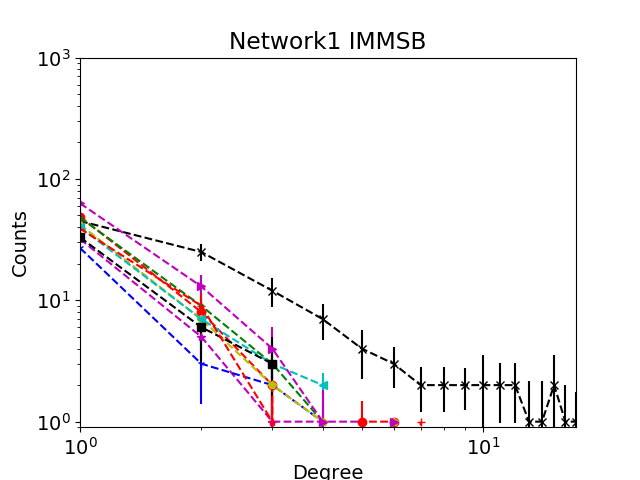
\includegraphics[width=\textwidth]{img/corpus/immsb_network1_1}
        \end{minipage}
        \begin{minipage}{0.24\textwidth}
            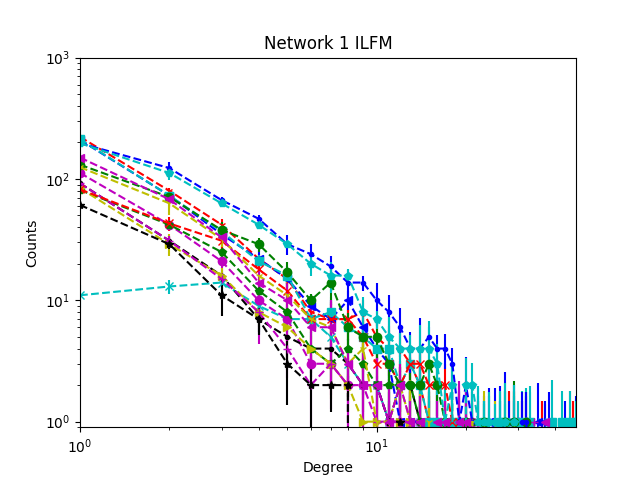
\includegraphics[width=\textwidth]{img/corpus/ilfm_network1_1}
        \end{minipage}
        \vskip\baselineskip
        \begin{minipage}{0.24\textwidth}
            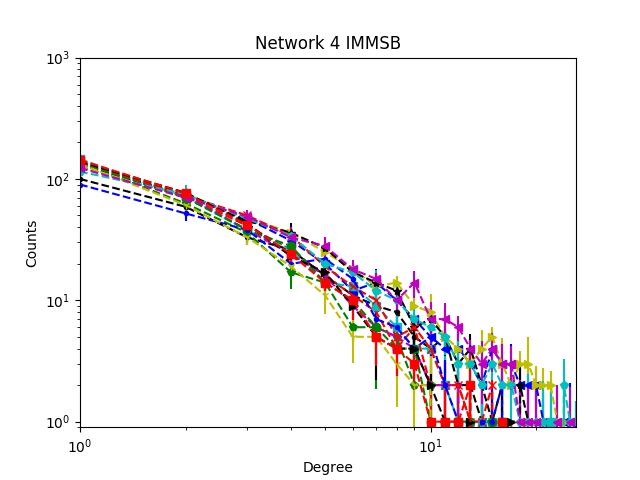
\includegraphics[width=\textwidth]{img/corpus/immsb_network4_1}
        \end{minipage}
        \begin{minipage}{0.24\textwidth}
            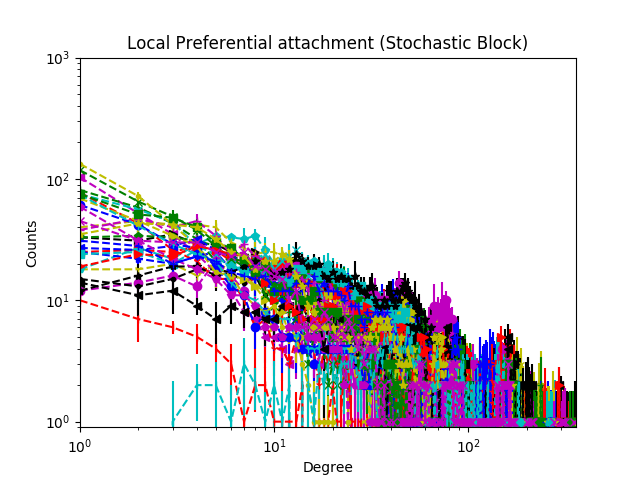
\includegraphics[width=\textwidth]{img/corpus/ilfm_network4_1}
        \end{minipage}
        \caption {Local degree distribution for of fitted models for Network 1 (first column) and Network 4 (second column) learned by IMMSB (row 1) and ILFM (row 2).} 
	\label{fig:me_local}
\end{figure}


\begin{figure}[h]
    \centering
        \begin{minipage}{0.24\textwidth}
            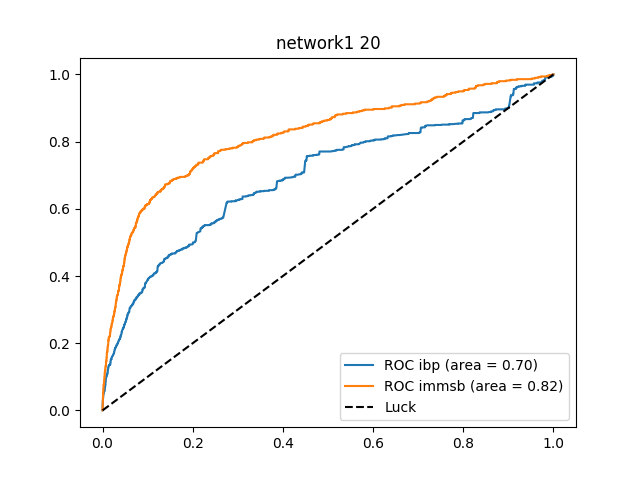
\includegraphics[width=\textwidth]{img/corpus/roc_network1_20}
        \end{minipage}
        \begin{minipage}{0.24\textwidth}
            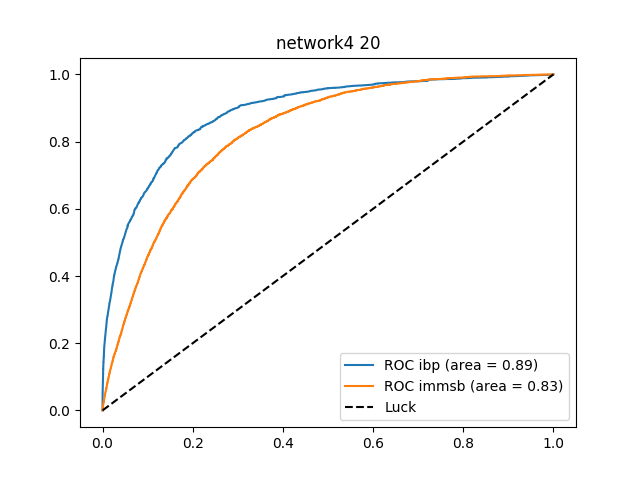
\includegraphics[width=\textwidth]{img/corpus/roc_network4_20}
        \end{minipage}
        \begin{minipage}{0.4\textwidth}
            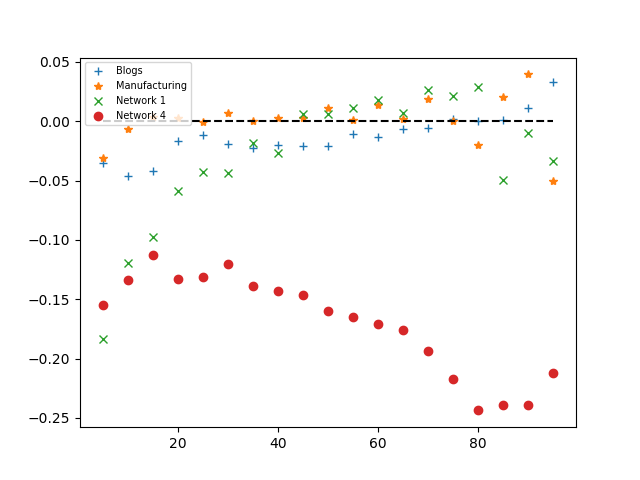
\includegraphics[width=\textwidth]{img/corpus/testset_max_20_roc_evolution.png}
        \end{minipage}
        \caption{The two upper top figures represent AUC-ROC curves that compares ILFM and IMMSB on network 1 and network4. The bottom figure is the relative AUC values when the size of the traning set vary. } 
	\label{fig:auc}
\end{figure}


In figure \ref{fig:auc} we report the AUC-ROC evaluation The two upper roc curves show a typical experiment for a bursty network (Network1) and a non bursty (Network 4). The figures show that IMMSB dominate ILFM on the first and is being dominated on the second. The bottom figure illustrate the relative performance of both models on each datasets for different ratio of the training size. The relative performance  is defined as the difference of the AUC value between IMMSB abd ILFM. The x-axis represents the following ratio $\frac{testset\ size}{training\ size}$. Hence the number of training data decrease in this graph. We shows that for bursty network, the relative performance of the prediction for IMMSB increase when the quantity of training data decrease. For non-bursty networks, the results is the opposite, the relative performance of ILFM increase when the size the training data decrease. This is particularly visible for Network4. For manufacturing this is more contrasted, probably due to the fact that the size of this networks is quite small which make the comparison more difficult.


\begin{figure}[h]
    \centering
        \begin{minipage}{0.24\textwidth}
            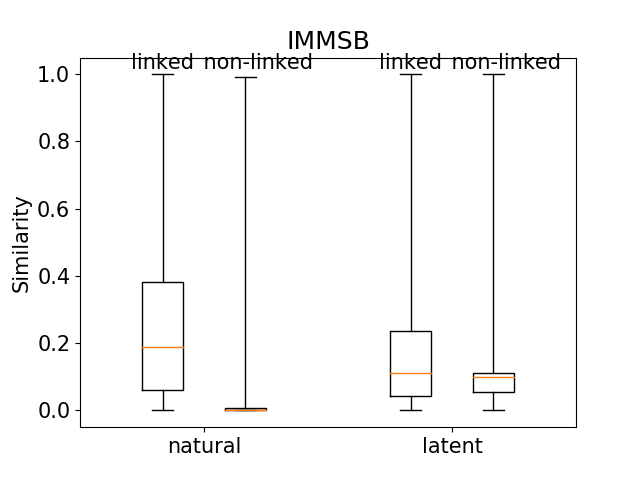
\includegraphics[width=\textwidth]{img/corpus/homo_mustach_immsb}
        \end{minipage}
        \begin{minipage}{0.24\textwidth}
            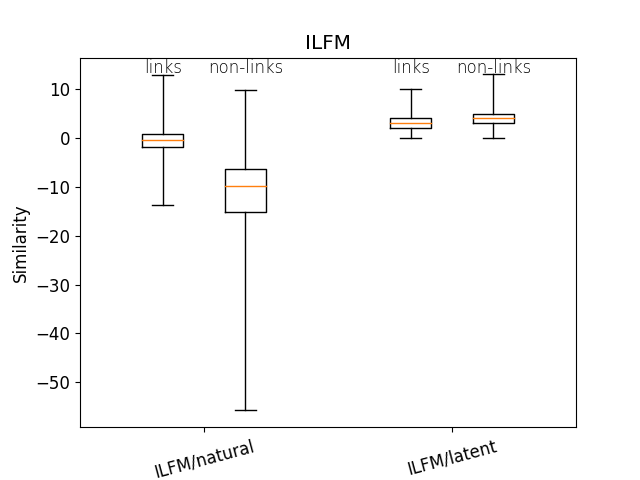
\includegraphics[width=\textwidth]{img/corpus/homo_mustach_ilfm}
        \end{minipage}
        \caption{Box plot for IMMSB (left) and ILFM (left) of the distribution for natural and latent similarity on the overall datasets. }
        \label{fig:homo_mustach}
\end{figure}

In figure \ref{fig:homo_mustach} we report the homophily measure. The left and right figures represent respectively the distribution of similarities for IMMSB and ILFM. It confirms that the natural similarities are statistically higher for the links than the non-links for both models but for IMMSB non-links similarities are more concentrated around zeros which is an interesting insight of the bursty behavior of IMMSB. For the latent similarity we see that there is no evidence of correlation the similarities with either  the links and non-links. 

